%===================================== CHAP 4 =================================

\chapter{Experiment}

Introduce the experiment

\section{Dataset}
This section will introduce the dataset(s) used. What features it contains, what we try to learn/classify, and why we chose to use it.
The Spambase Dataset \cite{spambase1999data} was used as a baseline training set. This dataset is publicly available from the UCI machine learning directory, and contains 57 input attributes of continuous format which serves as input features for spam detection and 1 target attribute in discrete format which represents the class.

We chose this dataset as it is a popular dataset to analyze the performance of binary classifiers, so that we could compare the results of other logistic regression classifiers against our own. While this dataset might not seem like the ideal choice for testing a differentially private classifier due to its lack of personal information, we argue that it still fits well for the purpose of demonstration. In a spam-classifying system based on our distributed model, a logistic regression model can be built by training it locally in each user's personal mail folder and then aggregated into an ensemble. That way you can build a diverse spam-classifier without the users having to give up their personal email to a centralized database.     

Used normalization to scale the data to 0-1 range, this is due to the proof in Chaudhuri paper which states the assumption $|X_i|< 1$. Based on the formula
\begin{eqnarray}
	X_{norm} = \frac{X-X_{min}}{X_{max} - X_{min}}
\end{eqnarray}

\section{Parameter tuning}

Number of peers $P$ specifies how many different peers participate in the experiment, and necessarily the number of partitions of the training data sets. The training is divided into $P$ parts of equal size.

Aggregate models are created from local models at each peer through an aggregation process that is performed one or more times with subsets of peers. The parameter $g$ specifies how many peers will participate in a single model aggregation. Since each peer has a unique subset of data, this parameter determines how many partitions of the training set contribute to the published aggregate models. These data partitions do not contribute directly, but indirectly through the aggregation of models trained locally on each partition.

Each peer trains a local logistic regression classifier on its data partition. This requires selection of a learning rate $\alpha$, a regularization constant $\lambda$ and a maximum number of iterations of gradient descent $I$. The learning rate is sensitive to the size of the local training set\cite{wilson20013learningrate}, and should be tuned individually by each peer. In usual data mining applications the regularization $\lambda$ would be tuned in this manner as well, but the sensitivity of the aggregation mechanism depends on $\lambda$, as seen in Equation \ref{eq:aggregated_logistic_sensitivity}. This means that the peers will have to communicate to either agree on a regularization level or to determine the smallest regularization constant to identify the worst case noise level. In our experiments we chose a global regularization level, which was used by all peers. We identified the best $\lambda$ by testing a coarse grid of powers of 2 whenever we changed the per-peer number of training samples.

The privacy parameter $\epsilon$ determines the level of privacy for each data partition. Note that this parameter does not apply to the original training set as a whole - each peer has its own private database, which is protected by $\epsilon$-differential privacy. 

Finally, the parameter $\epsilon$ can be divided across several applications of the aggregation mechanism, as described in Section \ref{section:privacy_budget}. This was achieved with a per-aggregation parameter $\epsilon_i$. Each data partition can participate the aggregation mechanism $n$ times, where $n\epsilon_i \leq \epsilon$.

\todo{Insert logistic regression training algorithm including hyperparameter usage}

\section{Validation}

The test sets set aside could not be used when tuning and evaluating system hyperparameters. In order to explore the effects of the various hyperparameters we used cross validation with number of folds $n=10$. For a given combination of hyperparameters, performance metrics were measured as their average across ten repetitions. In repetition $i$, data fold $i$ was used as validation set and the remaining $n-1$ data folds were combined to form the test set.

For the XXXX experiment\todo{insert experiment here}, the test set was used.

\section{Algorithm}

This section explain the logistic regression algorithm, how it is commonly used, and what modifications are needed when used in a distributed setting. Explanation on how it is used in a differentially private manner is explained in the architecture section. 

\subsection{Platform Setup}

\subsection{Application of Aggregation Mechanism}

\begin{algorithm}[H]
	\KwIn{$P$ - the set of peers\;
		$\epsilon$ - privacy parameter\; 
		$\epsilon_A$ - privacy level of a mechanism application\;
		$A$ - the $\epsilon_A$-differentially private aggregation mechanism\;
		$g$ - number of peers in a single mechanism application}
	\For{peer $\in$ P}{
		$budget_{peer} \leftarrow \epsilon$\;
	}
	\While{$|P| \geq g$}{
		$G \leftarrow randomSample(P, g)$\;
		model $\leftarrow A(G)$\;
		\For{peer $\in$ G}{
			$budget_{peer} \leftarrow budget_{peer} - \epsilon_A$\;
			\If{$budget_{peer} < \epsilon_A$}{
				$P \leftarrow P \smallsetminus peer$\;
			}
		}
		$publish(P, model)$
}
\caption{Aggregation mechanism}
\end{algorithm}

\todo[inline]{Defend randomSample procedure using Newscast reference}

\subsection{Fitting Local Classifiers}

\begin{algorithm}[H]
	\KwData{Set of training samples $D$}
	\KwIn{$\lambda$ - regularization strength\;
		$\alpha$ - learning rate\; 
		$iterations_{max}$ - maximum number of iterations}
	\KwResult{Logistic regression model fitted to $D$}
	$model \leftarrow 	$
	\For{$iterations_{max}$ iterations}{
		repeat-block;\
		}
	\caption{Gradient descent of logistic regression model}
\end{algorithm}

\subsection{Propegation Of Published Models}

\unsure{Remove this subsection if propegation is not tested}

\subsection{Distribution}
Introduce notion of distributed machine learning. 

Why did we choose to perform distributed learning?

How does it fit with the notion of differential privacy?

Can we guarantee differential privacy while doing it distributed

Record-based differential privacy. Does it work?

\todo[inline]{This section should maybe go somewhere else, but where?}



\section{Architecture}

In this section we will describe the architecture of Archipelago, our distributed machine learning system. 
Using notions borrowed from PINQ, we designed a distributed system using the JADE framework. Consists of explanation of peers, NoisyQueryable, DataLoader

 \missingfigure[figwidth=6cm]{Figure explaining our framework}

\subsection{Experiment instantiation and reset}


\subsection{Communication}
\subsubsection{Peer}
How is each peer set up, and what behaviors do they implement? 
How do they update then propagate the model being learned.
How do they know when to stop?
\subsubsection{messaging}
How do the peers communicate with each other?
What does a message look like?
What is the PeerGraph?
What controls the messages and determines where they should go?
\begin{figure}[h!]
	\centering
	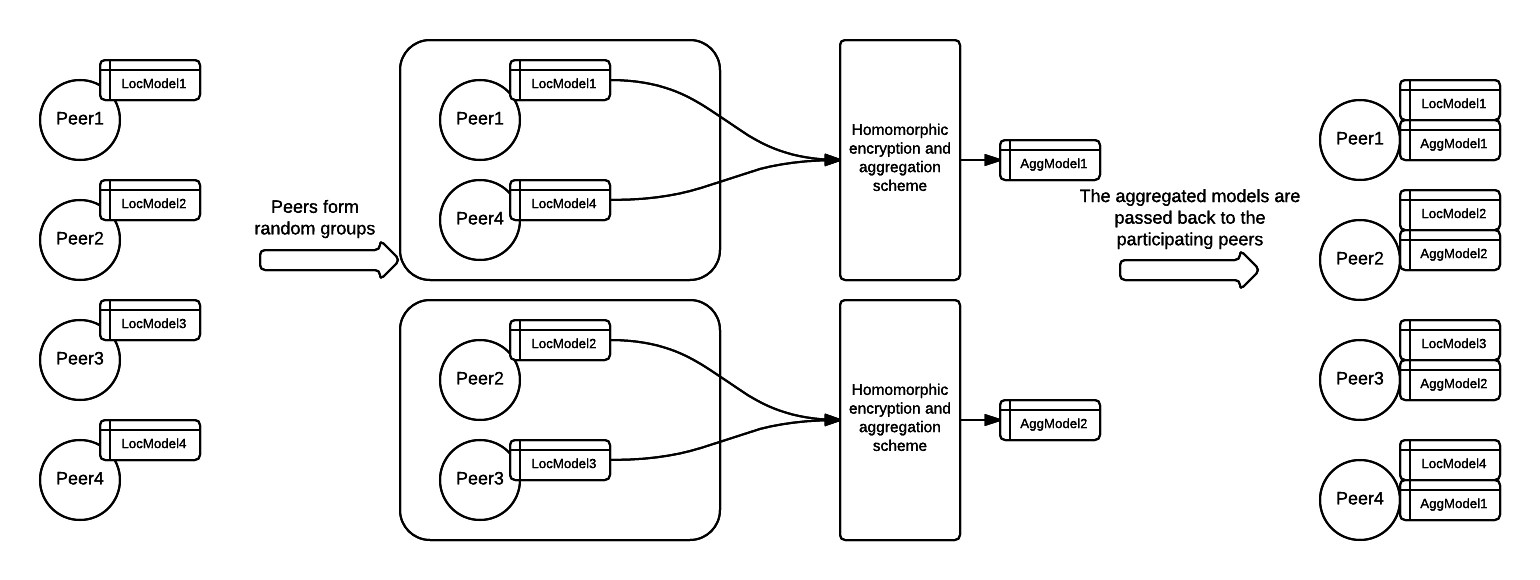
\includegraphics[width=\textwidth]{fig/peerModelCreation}
	\caption{One iteration of model aggregation}
	\label{fig:peerAggregationFigure}
\end{figure}


\subsection{Learning}
How is a logistic model implemented in our framework?

How is a model created and passed around the network?
Each Peer creates a logistic model based on their local data. They then form groups by calling the GroupFormingManager which assigns a group of peers together. This groups creates an aggregated model based on their own local ones. Here we simulate a Homomorphic Encryption scheme which assigns noise by secret sharing. 


How does the ensemble learning choose the best model?
What kind of performance metrics are used?
Mean classification error and Confusion Matrix.

\subsection{Privacy}
How does our framework guarantee differential privacy?
Based on the paper by 

\subsection{Experiment}
How are the experiments set up?
Explain the testing scheme.

Jade is re-run with while changing the initial parameters for the amount of peers, and the size of the groups they form. This test if performed over 10 iterations, while the mean classification error is recorded for each iteration. Each peer also create a confusion matrix with their classification results, and the peer with the best classification accuracy is saved and used to create a ROC-curve. 

Automatic testing scheme - Jade is configured so that it resets the main container after each experiment, and then re-run with new parameter configurations. 

Implemented 10-fold cross validation. This way we can tune the parameters and not be scared of our model overfitting on the test data. our initial solution was to use a single training and a single test set. This way we tuned the parameters so that they would give the best possible accuracy on the test set, which is not how the system should behave in the real world. 



\cleardoublepage